\normaltrue
\correctionfalse

%\UPSTIidClasse{12} % 11 sup, 12 spé
%\newcommand{\UPSTIidClasse}{11}

\exer{Mouvement T -- $\star$ \label{C2:091D:01}}
\setcounter{question}{0}\UPSTIcompetence[2]{C2-09}
\index{Compétence C2-09}
\index{Principe fondamental de la dynamique}
\index{PFD}
\index{Mécanisme à 1 translation}
\ifcorrection
\else
\marginnote{\textbf{Pas de corrigé pour cet exercice.}}
\fi

\ifprof
\else
Soit le mécanisme suivant. On note $\vect{AB}=\lambda(t)\vect{i_0}$. On note $m_1$ la masse du solide \textbf{1}.
On note $G$ le centre d'inertie de \textbf{1} tel que $\vect{BG}=\ell \vect{j_1}$. La pesanteur est telle que $\vect{g}=-g\vect{i_0}$. Un vérin positionné entre \textbf{1} et \textbf{0} permet d'actionner la pièce \textbf{1}. 
%On souhaite prendre en compte les frottements secs dans la liaison glissière.
%M et $\inertie{B}{1}=\matinertie{A_1}{B_1}{C_1}{-D_1}{0}{0}{\bas{1}}$.
\begin{center}
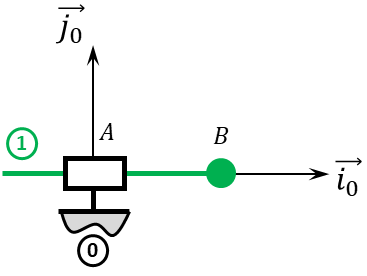
\includegraphics[width=.6\linewidth]{01_T_01}
\end{center}



Les performances dynamique de l'axe demandées sont les suivantes : 
\begin{itemize}
\item vitesse linéaire maximale : $50 \; \text{m}\,\text{min}^{-1}$;
\item accélération linéaire maximale : $9,8 \; \text{m}\, \text{s}^{-2}$.
\end{itemize}

\begin{obj}
L'objectif de ce travail est de déterminer les caractéristiques du moteur (vitesse et couple) permettant d'atteindre ces performances.
\end{obj}
\fi

\question{Quelle est la vitesse maximale que l'axe peut atteindre en  $\text{m}\, \text{s}^{-1}$.}
\ifprof
$V = \dfrac{50}{60} = \SI{0,83}{m.s^{-1}}$.
\else
\fi

\question{Combien de temps l'axe met-il pour atteindre la vitesse maximale ?}
\ifprof
$T_a =0,83/9,8 = \SI{0,08}{s}$.


\else
\fi

\question{Quelle distance l'axe parcourt-il pour atteindre la vitesse maximale ?}
\ifprof
Si on trace le profil de vitesse en fonction du temps, la distance parcourue correpond à << l'aire sous la courbe >>. 

On a donc $D_a = \dfrac{1}{2}T_a V  \simeq \SI{0,03}{m}$. 

\else
\fi


\question{Quelle est la longueur minimale à commander pour que l'axe puisse atteindre la vitesse maximale ?}
\ifprof
Pour atteindre la vitesse maximale, il faut donc commander une distance supérieure à \SI{0,06}{m}.
\else
\fi

%\question{Proposer une longueur minimale de l'axe pour pouvoir profiter de ses performances dynamiques.}
%\ifprof
%
%\else
%\fi

\question{Tracer le profil de la position, de la vitesse et de l'accélération pour parcourir une distance de 50 cm. On cherchera à atteindre les performances maximales de l'axe. }
\ifprof

\else
\fi

\ifprof
\else

Un motoréducteur permet d'entraîner un système poulie -- courroie permettant de déplacer la charge. On considère :
\begin{itemize}
\item une charge de masse $1\; \text{kg}$;
\item un poulie de rayon $5\; \text{cm}$;
\item un réducteur de rapport de transmission $1:20$.
\end{itemize}

\begin{center}
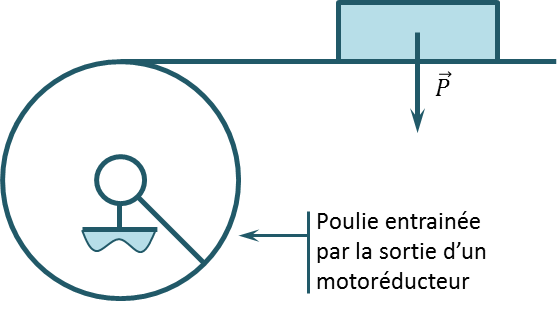
\includegraphics[width=.9\linewidth]{fig_12}
\end{center}

\fi

\question{Déterminer le couple à fournir par la poulie pour déplacer la charge lorsque l'accélération est au maximum. }
\ifprof

\else
\fi

\ifprof
\else
\begin{flushright}
\footnotesize{Corrigé  voir \ref{C2:091D:01}.}
\end{flushright}%
\fi


